\documentclass[12pt]{article}

\usepackage[left=25mm, top=30mm, bottom=20mm, right=25mm, headsep=10mm]{geometry}
\usepackage[utf8]{inputenc}
\usepackage[german]{babel}
\usepackage{fancyhdr}
\usepackage{graphicx}
\usepackage{color, colortbl}
\usepackage{tabularx}
\usepackage{helvet}
\usepackage[table,xcdraw]{xcolor}
\usepackage{enumitem}
\usepackage{parskip}
\usepackage{float}

\setlength{\parindent}{0pt}

\newcommand{\subsubsubsection}[1]{\paragraph{#1}\mbox{}\\}
\setcounter{secnumdepth}{4}
\setcounter{tocdepth}{4}

% ============== START Header and Footer ============== %
% http://tug.ctan.org/info/german/fancyhdr/fancyfolien+bsp.pdf
\pagestyle{fancy}
\renewcommand{\headrulewidth}{.5pt}
\fancyhead[OL,EL]{\fontsize{9}{12} \selectfont Advanced Data Managment}
\fancyhead[OR,ER]{\fontsize{9}{12} \selectfont Redis Intro}

\renewcommand{\footrulewidth}{.5pt}
\fancyfoot[OL,EL]{\fontsize{9}{12} \selectfont Berner Fachhochschule}
\fancyfoot[OC,EC]{\fontsize{9}{12} \selectfont \thepage}
\fancyfoot[OR,ER]{\fontsize{9}{12} \selectfont Lars Peyer, Adrian Berger}
% ============== END Header and Footer ============== %

\makeatletter
\setlength{\@fptop}{0pt}
\makeatother

\begin{document}
	
	\begin{titlepage}
	
	\begin{center}
		
\includegraphics[width=100mm]{media/titleimage.jpg}\\[10mm]	
		\line(1,0){450}\\[7mm]
		\huge{Advanced Data Management \protect\\[10mm] Redis Intro}\\[2mm]
		\line(1,0){450}\\[2cm]
		\large{Peyer Lars}\\[3mm]
		\large{Berger Adrian}\\[15mm]
		\large{Version 1.0}\\[5mm]
		\today\\[20mm]
		
	\end{center}
\end{titlepage}
\newpage
	\renewcommand{\contentsname}{\vspace{-1.5cm}}
\tableofcontents
\newpage
	\section{Key Value Store}
\subsection{Definition}
Ein Key Value Store basiert auf einer Tabelle mit genau zwei Spalten: \\
In der einen befindet sich ein eindeutiges Identifikationsmerkmal, der Schlüssel (Key), in der anderen der Wert (Value).
Somit wird jeder Wert eindeutig einem Schlüssel zugewiesen.
Welche Datentypen im Wert gespeichert werden können, ist abhängig vom verwendeten Key-Value Store.
Es handelt sich somit um eine NoSQL Datenbank.
\subsection{Vorteile und Nachteile}
\subsubsection{Vorteile}
\begin{itemize}
	\item Geschwindigkeit
	\item Skalierbarkeit
	\item Simples Model, einfach verständlich
\end{itemize}
\subsubsection{Nachteile}
\begin{itemize}
	\item Für Daten mit vielen relationalen Abhängikeiten sehr komplex
	\item Keine Lookup Optimierungen für das Suchen
\end{itemize}
\subsection{Einsatzgebiete}
Überall wo schnelle Zugriffszeiten bei großen Datenmengen benötigt werden, eignen sich Key Value Stores. Typische Einsatzgebiete sind deshalb Warenkörbe in Onlineshops oder das Speichern von Session-Daten.

\subsection{In-Memory}
Bei vielen Key Value Stores handelt es sich um In-Memory Datenbanken. Im Gegensatz zu herkömmlichen On-Disk Datenbanken verwenden diese anstelle des ROM, den Arbeitspeicher eines Computers.

\begin{table}[H]
	\begin{tabular}{|p{1.6cm}|p{4.6cm}|p{4.6cm}|p{4.6cm}|}
		\hline
		\rowcolor{black}
		&
		\textcolor{white}{\textbf{Disk}} & \textcolor{white}{\textbf{SSD}} &
		\textcolor{white}{\textbf{In-Memory}}
		\\
		Funktion & rotierenden Magnetscheiben & Flash-Speicherchips & In-Memory\\ 
		\hline
		Stärken & Priorität & Muss & Test \\
		\hline
		Grenzen & 7200 RPM (BarraCuda Pro) & Muss & Test \\
		\hline
		Weiteres & Priorität & Muss & Test \\
		\hline 
	\end{tabular}
\end{table}

Disk und SSD - Charakteristiken, Stärken und Grenzen
Die Bedeutung von In Memory Datenbanken

\subsection{Top 5 Key Value Stores}
Gemäss db-engines.com (Stand 27.10.2019) sind die folgenden Datenbanksysteme führend:
\begin{enumerate}
\item Redis
\item Amazon DynamoDB
\item Microsoft Azure Cosmos DB
\item Memcached
\item Hazelcast
\end{enumerate}

	\clearpage
	\section{Redis}
\subsection{Charakterisierung}
Redis ist ein Open Source, In-Memory Datenbanksystem, das als vorallem als Datenbank, Cache und Message Broker verwendet werden kann.\\
Redis ist BSD lizenziert und stellt somit keine Anforderungen an die Weiterverteilung der Software.\\
Der Name Redis entstand als Abkürzung für remote dictionary server.\\
Entwickelt wurde Redis 2009 von Salvatore Sanfilippo in C und gehört mitlerweile zu VMWware. Die aktuelle Version (Stand 5. November 2019) ist 5.0.5, wobei die aktuelle LTS Version 3.2.11 ist.
Redis ist single-threaded und lässt sich einfach replizieren.

\subsubsection{Platformen, welche Redis verwenden}
Redis erfreut sich grosser Beliebtheit und ist laut DB-Engines.com die verbreitetste Key-Value Datenbank.
Einige der grossen Kunden sind etwa Twitter (Real-Time Delivery), Github (Speicherung von Routing Information) und StackOverflow (2-Level Cache).\\
Mehr Infos unter: https://redis.io/topics/whos-using-redis
\subsection{Installation}
Redis lässt sich leicht als tar.gz gerunterladen und installieren:
\begin{lstlisting}[language=bash]
wget http://download.redis.io/redis-stable.tar.gz
tar xvzf redis-stable.tar.gz
cd redis-stable
make
make install
\end{lstlisting}
Mehr Infos unter: https://redis.io/topics/quickstart
\clearpage
\subsection{Datentypen}
Redis unterstützt die folgenden Datentypen:
\begin{table}[H]
	\begin{tabular}{|p{3cm}|p{12.7cm}|}
		\hline
		\rowcolor{black}
		\textcolor{white}{\textbf{Typ}} &
		\textcolor{white}{\textbf{Beschreibung}}\\
		
		String & Eine beliebige Zeichenfolge\\ 
		\hline
		List & Entspricht einem Array, die Elemente werden über einen positiven, ganzzahligen, null-basierten Index angesprochen \\
		\hline 
		Hash & Entspricht einem assoziativem Array, die Elemente bestehen hier wiederum aus Schlüssel-Werten Paaren.\\
		\hline 
		Set & Wie List, jedoch kann jedes Element nur einmal vorkommen darf.\\
		\hline 
		Sorted Set & Entspricht einem Set, nur dass zusätzlich der Index des Elements explizit mit angegeben wird.\\
		\hline 
		Bitmaps & Speicherung von Bits\\
		\hline 
		HyperLogLogs & Probabilistische Datenstruktur, mit der sich die Kardinalität einer Datenmenge sehr speichereffizient bestimmen lässt\\
		\hline
	\end{tabular}
\end{table}
Mehr Infos unter: https://redis.io/topics/data-types
\subsection{Abfragesprache}
Für String lässt sich ein Speichern und Abrufen mit get und set erreichen (alle Beispiele mit Python Redis):
\begin{lstlisting}[language=python]
import redis
r = redis.Redis()
r.set("msg:hello", "Hello Redis!!!")
msg = r.get("msg:hello")
# prints b'Hello Redis!!!'
\end{lstlisting}

Für jeden Datentyp gibt es solche Schreib- und Lesebefehle. Zudem gibt es diverse weitere Befehle (z.B. zum Zählen der Elemente). Nachfolgend ein Beispiel für ein Set:
\begin{lstlisting}[language=python]
mountainSet = "Berge"
# Add elements to the Redis set
r.sadd(mountainSet, "Eiger")
r.sadd(mountainSet, "Moench")
r.sadd(mountainSet, "Jungfrau")

print("Anzahl Elmente: ")
print(r.scard(mountainSet))
print(r.smembers(mountainSet))
# prints Anzahl Elmente: 3 {b'Eiger', b'Moench', b'Jungfrau'}
\end{lstlisting}
Eine Liste aller Abfragen findet sich hier: https://www.cheatography.com/tasjaevan/cheat-sheets/redis/
\subsubsection{Transaktionen}
Eine Transaktion in Redis besteht aus einem Block von Befehlen, die zwischen MULTI und EXEC (oder DISCARD für Rollback) platziert werden. Sobald ein MULTI gefunden wurde, werden die Befehle auf dieser Verbindung nicht ausgeführt - sie stehen in der Warteschlange (und der Anrufer erhält die Antwort QUEUED). Wenn eine EXEC angetroffen wird, werden sie alle in einer einzigen Transaktion angewendet (d.h. ohne dass andere Verbindungen Zeit zwischen den Operationen erhalten). Wenn anstelle von EXEC eine DISCARD gesehen wird, wird alles weggeworfen. Da die Befehle innerhalb der Transaktion in der Warteschlange stehen, können Sie innerhalb der Transaktion keine Entscheidungen treffen.

Sämtliche Informationen dazu finden sich hier: https://redis.io/topics/transactions

\subsection{Massenload}
Manchmal müssen Redis-Instanzen in kurzer Zeit mit einer großen Menge an bereits vorhandenen oder benutzergenerierten Daten geladen werden, sodass Millionen von Schlüsseln so schnell wie möglich erstellt werden.

Ab Redis 2.6 unterstützt das Dienstprogramm redis-cli einen neuen Modus namens Pipe-mode, der entwickelt wurde, um eine Masseneinfügung durchzuführen.

Die genaue Spezifikation dazu findet sich hier: https://redis.io/topics/mass-insert

\subsection{Benchmarks}
Redis bietet das Dienstprogramm redis-benchmark, das laufend Befehle von Clients simuliert und gleichzeitig Gesamtabfragen sendet. Damit kann die Performance von Redis getestet und visualisiert werden.\\
Anleitungen und Beispiele dazu finden sich hier: https://redis.io/topics/benchmarks

\subsection{API}
Redis-Module sind dynamische Bibliotheken, die beim Start oder mit dem Befehl MODULE LOAD in Redis geladen werden können.

Redis-Module ermöglichen es, die Redis-Funktionalität durch externe Module zu erweitern, indem sie neue Redis-Befehle mit einer Geschwindigkeit und mit ähnlichen Funktionen implementieren, wie sie im Kern selbst möglich sind.

Weiter Informationen dazu finden sich hier: https://redis.io/topics/modules-intro
\clearpage
\subsection{Persistenz}
Redis bietet generell zwei Varianten der sicheren Datenspeicherung:

RDB (Snapshots): Zu bestimmten Zeitpunkten (z.B. jede volle Stunde) wird eine vollständige Kopie der im Speicher befindlichen Daten erstellt. Wenn z.B. zwischen zwei Snapshots die Stromversorgung verloren geht, gehen die Daten aus der Zeit zwischen dem letzten Snapshot und dem Crash verloren. 

AOF: Logt jede vom Server empfangene Schreiboperation und führt diese beim Serverstart erneut ab zur Rekonstruktion des ursprünglichen Datensatzes.

Grundsätzlich lassen sich RDB und AOF einzel aktiviren. Somit wäre auch keine Persistenz möglich, in dem beides deaktiviert wird. Die beste Persistenz wird erreicht, in dem beides aktiviert wird. Grundsätzlich handelt es sich hierbei um eine Frage zwischen Datensicherheit und Leistung.\\

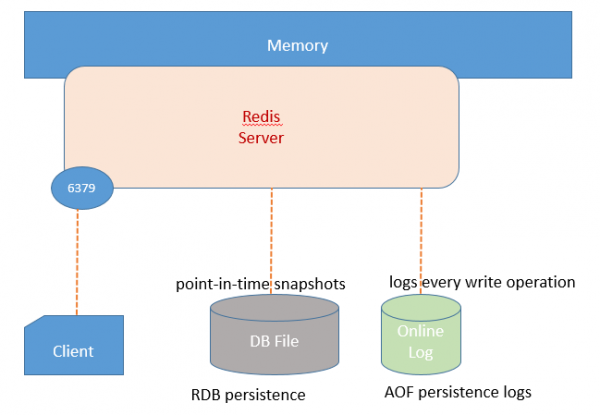
\includegraphics[width=160mm]{media/redis.png}\\[10mm]	
Weitere Vor- und Nachteile finden sich hier: https://redis.io/topics/persistence
\clearpage
\subsection{Replikation}
Auf der Basis der Redis-Replikation gibt es eine sehr einfach zu bedienende und zu konfigurierende Master-Slave-Replikation. Sie ermöglicht es, dass Redis-Instanzen als Replikate exakt von Master-Instanzen kopiert werden.

Dieses System arbeitet mit drei Hauptmechanismen:
\begin{enumerate}
\item Wenn Master und Slave verbunden sind, hält der Master den Slave auf dem neuesten Stand, indem er einen Befehlsstrom sendet, um die Auswirkungen auf den Slave Datensatz zu replizieren.
\item Wenn die Verbindung zwischen Master und Slave abbricht, verbindet sich der Slave erneut und versucht, mit einer teilweisen Resynchronisierung fortzufahren: Er erhäötn nur den Teil des Befehlsstroms, den er während der Trennung verpasst hat.
\item Wenn eine teilweise Resynchronisation nicht möglich ist, fordert der Slave eine vollständige Resynchronisation an. Dies erfordert einen komplexeren Prozess, bei dem der Master einen Snapshot aller seiner Daten erstellen, an den Slave sendet.
\end{enumerate}
Redis verwendet standardmässig asynchrone Replikation, die eine geringe Latenz und hohe Leistung aufweist. Redis-Slaves bestätigen jedoch asynchron die Menge der Daten, die sie periodisch vom Master empfangen haben. Der Master wartet somit nicht jedes Mal darauf, dass ein Befehl von den Replikaten verarbeitet wird, weiß aber bei Bedarf, welcher Slave bereits welchen Befehl verarbeitet hat.

Redis lässt sich zudem mittels Redis Cluster auf mehrere Knoten verteilen.

Redis Cluster bietet die Möglichkeit den Betrieb fortzusetzen, wenn einige Knoten ausfallen oder nicht kommunizieren können. Bei größeren Ausfällen (z.B. wenn die Mehrheit der Master nicht verfügbar ist) stoppt der Cluster jedoch den Betrieb.


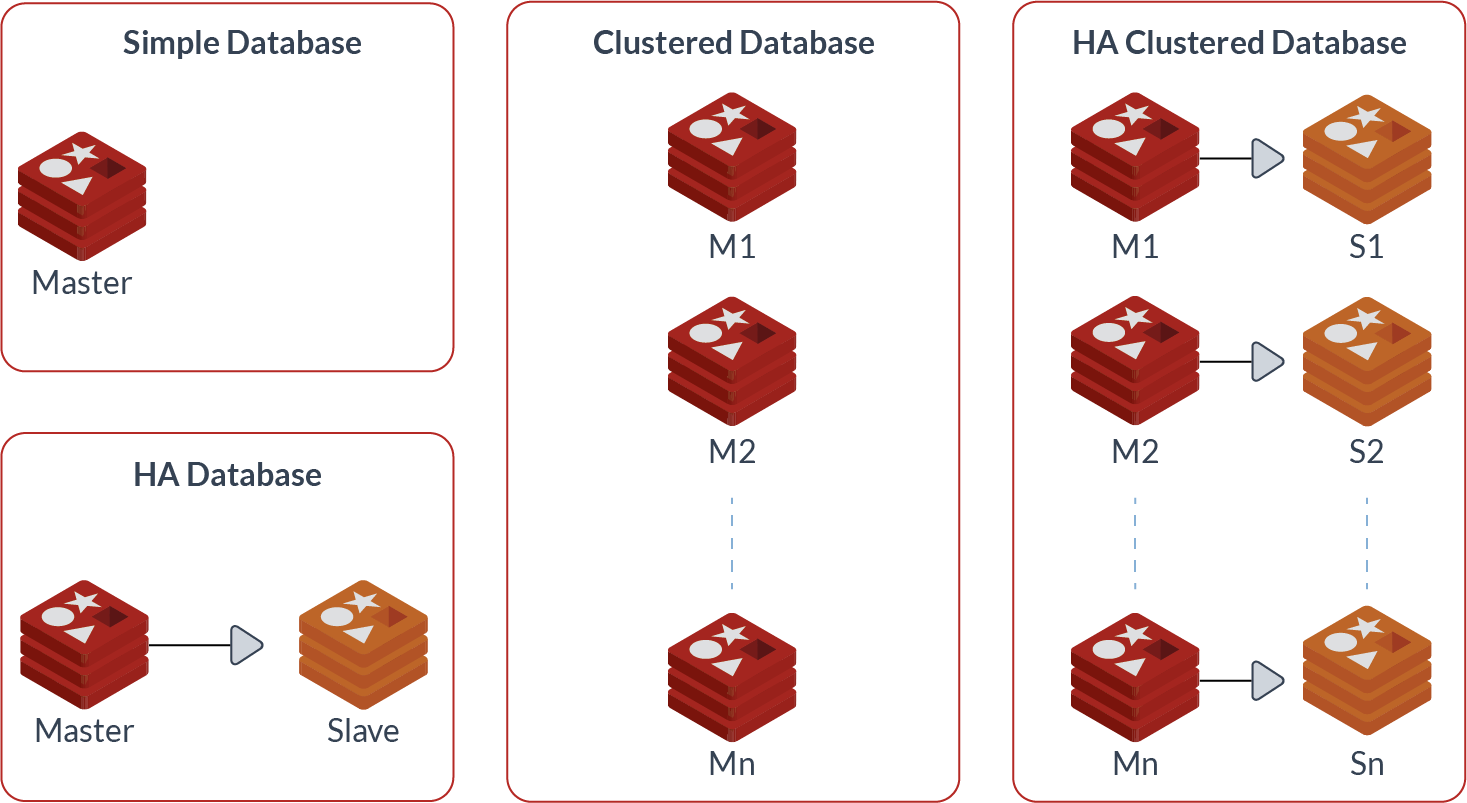
\includegraphics[width=140mm]{media/diagram-cluster-architecture.png}\\[5mm]	
Die Dokumentation dazu fndet sich hier: https://redis.io/topics/replication
\subsection{Optimierungsmöglichkeiten}
\subsubsection{Performance}
Mit Piplines kann die Performance verbessert werden, da nicht bei jeder Anfrage auf das Resultat vom Server gewartet wird, bis die nächste Anfrage gestartet wird. Somit laufen mehrere Abfragen gleichzeitig.
Mehr dazu findet sich hier: https://redis.io/topics/pipelining

Zudem kann die Performance optimiert werden, in dem RBD und AOF ausgeschalten werden. Dadurch geht jedoch auch das persistieren der Daten verloren.

\subsubsection{Memory}
Daten sollten immer, wenn es möglich ist, mit Hashes dargestellt werden, damit Memory gespart werden kann. So kann anstelle verschiedener Schlüssel ein einzigr Hash mit allen erforderlichen Feldern verwendet werden.

Zudem kann Redis auf 32 Bit umgestellt werden. Redis kompiliert mit 32-Bit verbraucht viel weniger Speicher pro Schlüssel, da die Zeiger klein sind, ist aber auf 4 GB maximale Speichernutzung beschränkt. RDB- und AOF-Dateien sind zwischen 32-Bit- und 64-Bit-Instanzen kompatibel.

Weitere Optimierungen finden sich hier: https://redis.io/topics/memory-optimization
\subsection{GUI}
Die bekanntesten und verbreitetsten GUIs für Redis sind: Redsmin, Redis Commander, Redis Desktop Manager und redis-browser.\\
Eine gute Übersicht findet sich hier: https://redislabs.com/blog/so-youre-looking-for-the-redis-gui/

\clearpage
\section{Ressourcen}
https://en.wikipedia.org/wiki/Key-value\_database\\
https://db-engines.com/de/ranking/key-value+store\\
https://www.aerospike.com/what-is-a-key-value-store/\\
https://www.ionos.de/digitalguide/hosting/hosting-technik/key-value-store/\\
https://redis.io/\\
https://redislabs.com\\
https://www.pipperr.de/dokuwiki/doku.php?id=nosql:redis\_overview\\
https://wikipedia.org/wiki/Redis\\
https://stackoverflow.com/questions/51314487/redis-memory-optimization-suggestions\\
	
\end{document}
